\documentclass{llncs}

\usepackage{amsmath,amssymb}
\usepackage{alg}
\usepackage{booktabs}
\PassOptionsToPackage{hyphens}{url}\usepackage{hyperref}
\usepackage{graphicx}
\usepackage{subfigure}
\usepackage{xspace}
\usepackage{color}

\Urlmuskip=0mu plus 1mu

\renewcommand\dblfloatpagefraction{.99}
\renewcommand\dbltopfraction{.9}
\renewcommand\floatpagefraction{.99}
\renewcommand\topfraction{.9}

\newcommand{\name}{\texttt{G-NPM}\xspace}
\newcommand{\npm}{\texttt{NPM}\xspace}
\newcommand{\todo}[1]{\texttt{\color{red}TODO:#1}}
\begin{document}


\title{G-NPM: Local Citation Recommendation System with Global Features}

\author{Byeonghyeon You, Seongmin Lee, Junbeom Lee, Jinhan Kim}

\institute{Korea Advanced Institute of Science and Technology\\Republic of Korea}

\maketitle

\begin{abstract}
\todo{JB}

\end{abstract}

\section{Introduction}
\label{sec:introduction}
As academic communities have published about the millions of research papers, finding appropriate citations become burdensome for researchers. Citation recommendation systems[] have cut down the overload of finding citations by automatically suggesting papers which might be related to the topic.


There are two main categories in citation recommendation, global and local citation recommendataion.
The first category, global citation recommendation, recommends a list of candidate papers by examining some part of the entire paper. In addition to exmaine the text, global citation recommendation systems use the external features such as information of author, venue, citation count, and h-index. These external features can make recommendation model more accurate.
The second category, local citation recommendation, recommends a list of candidate papers by just looking a sentence which is called citation context. Local citation recommendation systems only take citation context as an input, suggest papers which is relevant to that context. Intuitively, it is more practical to use than global citation recommendation systems.


Although the current state-of-the-art local citation recommendation system[] outperformed other approaches[], it showed relatively poor in recommending well-cited papers. Since global and local has own advantages, in this project, we propose the new citation recommendation system which is local citation recommendation system with global external features. We use citation count as a global external feature.


\section{Background}
This section describes the two citation recommendation models.

\subsection{Neural Probabilistic Model}
Neural Probabilistic Model, \npm ~\cite{Huang:2015:NPM:2886521.2886655}

NPM(Neural Probabilistic Model) is local citation recommendation model that learns the citing paper with given citation contexts. Training is separated into two parts, word representation learning and document representation learning. To learn words, they used negative sampling[] that is used to learn the distribution of words. To learn documents with words, they used noise-contrastive estimation[] that is used to learn the distribution of words and documents.

\subsection{Literature Search Model}
Literature Search Model~\cite{Bethard:2010:ICL:1871437.1871517}

\section{\name: A new citation recommendation system}
\todo{SM}


\section{Experiments}
\subsection{Research Questions}
\todo{SM}

\begin{enumerate}
\item Does G-NPM use global information(citation count) to improve the efficiency of citation recommendation system?
\item Is the G-NPM a model that can be applied competently on systems with small input data?
\end{enumerate}
\subsection{Setup}
\label{sec:setup}
For all experiments we used the same data set used in [2] which is a snapshot of Citeseer paper and citation database was obtained at Oct, 2013. The data is composed of three tables with unprocessed SQL data(90GB): citation table, citation context table, paper table. The citation table consists of cited paper id and citing paper id. The citation context table consists of the cited paper id and its context. One citation context consists of the sentence where a citation appears, as well as the sentences that appear before and after. The paper table consists of paper id. As a result, all the data set contains about 10,000,000 contexts and about 1,000,000 unique papers.
It took 4 days to only import the data set and we could not used as much resources as they[2] used for their experiments. Therefore, we randomly extracted 1 from the original data. The training data is consisted of 10520 contexts and 5613 cited papers. As test data, 999 contexts and corresponding 359 papers were randomly selected and tested.


Table 1

For text normalization, rare words that appear less than 5 times are filtered out and we did not distinguish between uppercase/lowercase words. In all experiments, we use the citation contexts and cited papers extracted from the test set as ground truth. Unlike the target paper the number of recommendations is not limited to 10 for each query because we only trained small amount of data which is causing less effective recommendation performance.

\subsection{Evaluation Metric}
\label{sec:metric}
We used 3 well-known metrics which are average rank, average rank at 10 and Mean Reciprocal Rank(MRR) on the information retrieval system to evaluate the ranking obtained from G-NPM. Average rank is the average value of recommended ranking. The rank means the order of the papers that are likely to be recommended. Average ranking at 10 is the average value of recommended ranking where the appropriate cited paper was assigned within top 10. The MRR is a statistic measure for evaluating any process that produces a list of possible responses to a sample of queries, ordered by probability of correctness. The reciprocal rank of a query response is the multiplicative inverse of the rank of the first correct answer.


\section{Results}

\subsection{Effectiveness}
Running experiment in Section~\ref{sec:setup}, \npm is able to rank documents to cite for 357 contexts out of 1,000 contexts test data. For remaining 643 contexts, \npm failed to rank documents to cite. Since the size of the training data is small, \npm can not learn the context sufficiently, resulting in a ranking failure for the test data. Even if \npm fails to rank documents, when we consider the \npm score to be 0, \name can still yield a valid score. Since the score of 643 data only reflects the global feature, it did not match the scope of our research: local citation recommendation. Therefore these data were excluded from the \npm and \name comparisons.

\begin{table}[ht]
\centering
\begin{tabular}{l || p{0.3 \textwidth} | p{0.3 \textwidth}}
\toprule
& \npm & \name \\
\midrule
Average rank$^\ast$ & 55.09 & 36.18 \\
Accuracy at 10 & 26 & 53 \\
MRR & 0.035 & 0.084\\
\midrule
\multicolumn{3}{l}{$\ast$: Lower value represents better results} \\
\bottomrule
\end{tabular}
\caption{Evaluation of \npm and \name ranking}\label{table:rq1}
\end{table}

Table~\ref{table:rq1} contains the ranking results of \npm and \name. As mentioned in Section~\ref{sec:metric}, the lower the Average rank, the better. Average Rank of \npm was 55, while  that of \name was 30. It means that we have to see 55 paper to find a relevant paper in \npm. But in \name, the human's reading efforts drops to 30. This cuts human efforts in half. For accuracy at 10. \npm placed the relevant paper in top ten in 26 cases, while \npm locates 53 papers. \name is twice more effective than \npm. Finally in MRR, \name recorded 0.084, but \npm recorded 0.035

\begin{figure}[ht]
\centering
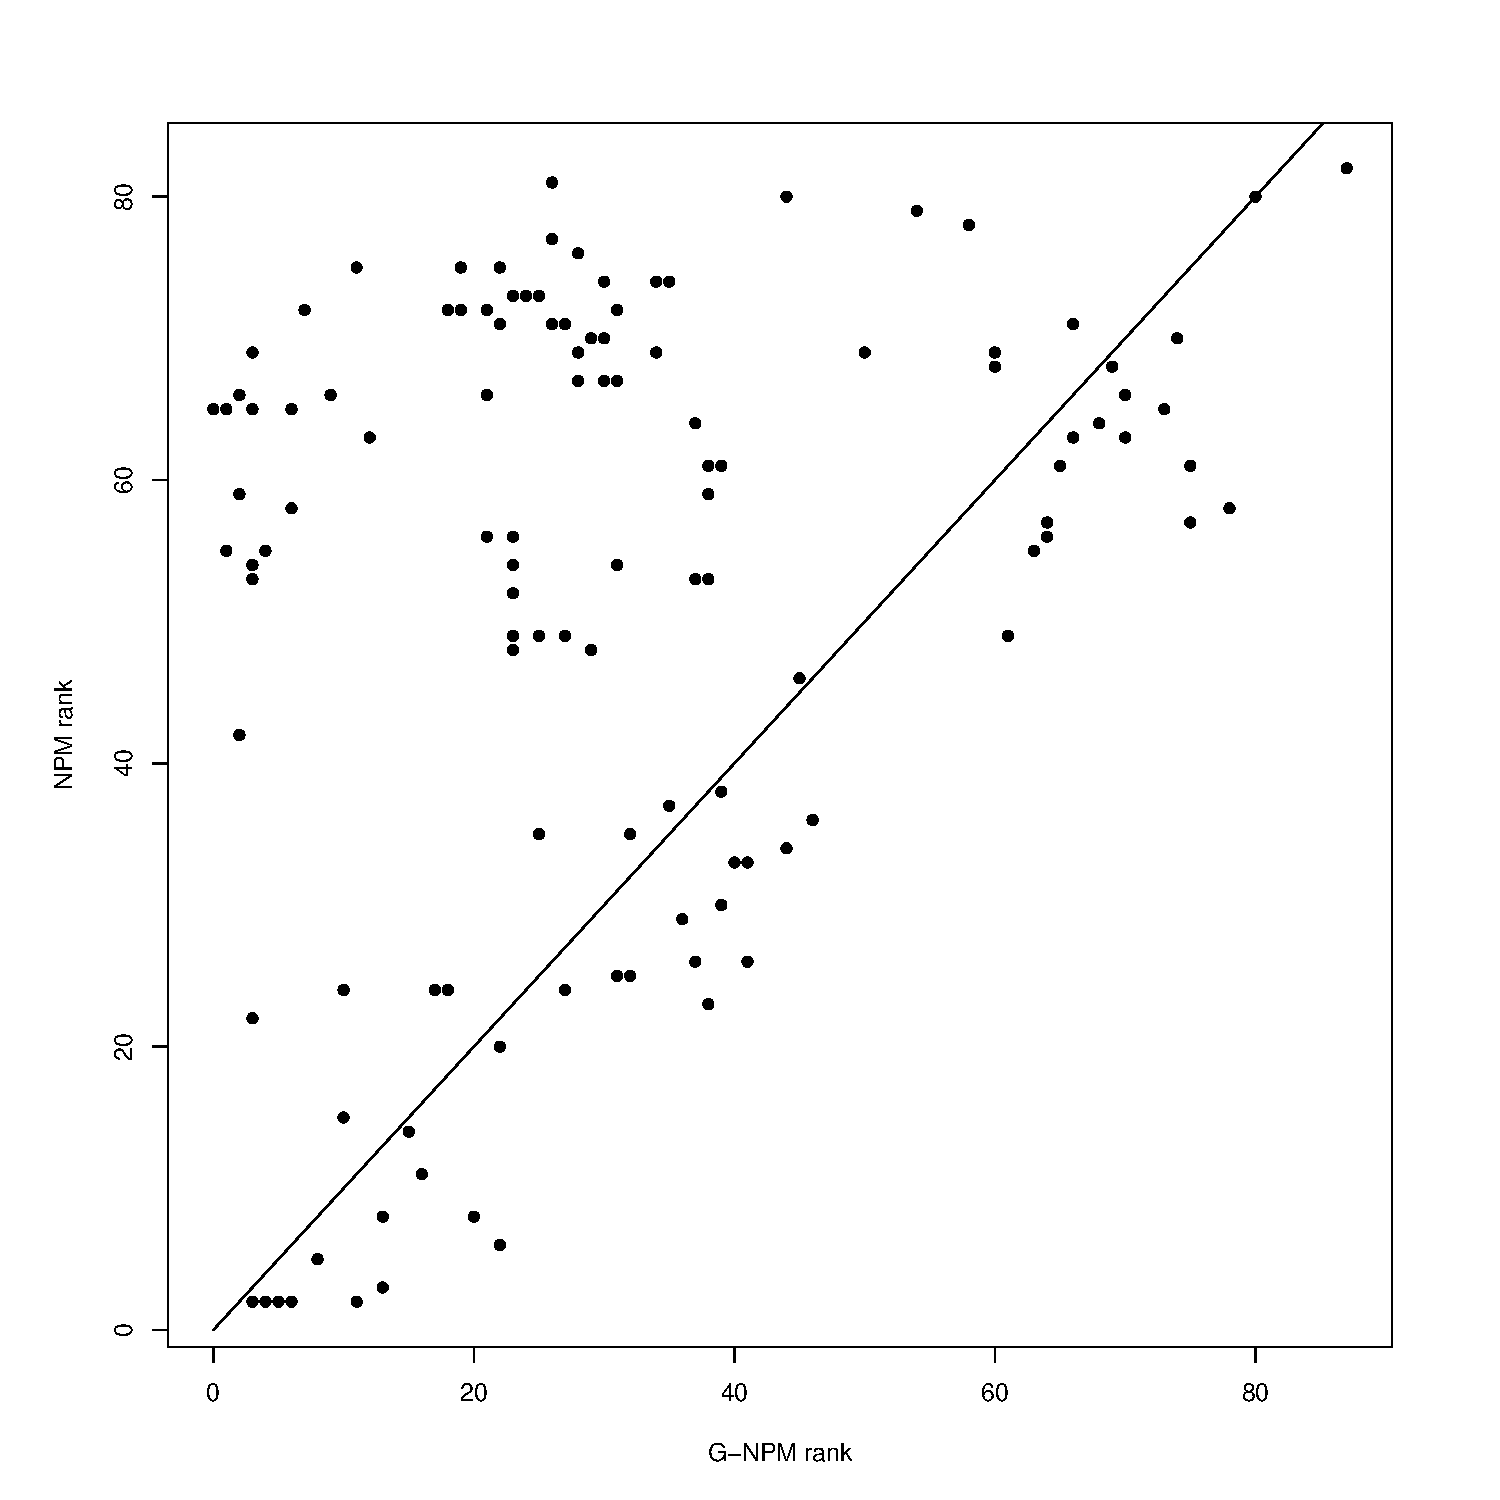
\includegraphics[width= 0.7\textwidth]{rq1.pdf}
\caption{Ranking Result of \name and \npm \label{fig:rq1}}
\end{figure}

Figure~\ref{fig:rq1} shows the ranking results visually. The X-axis is the ranking of relevant papers from \name and the Y-axis is the ranking of relevant papers from \npm. Clearly, the upper left part of the graphs shows the improvements of \name over \npm and the lower right area represents the negative cases which \name ranks worse than \npm. he number of positive cases is more than twice the number of negative cases. There were 248 positive cases and 107 negative cases. Furthermore, The ranking changes of positive cases were much greater than the ranking changes of negative cases. It means, in most of the cases, human effort to find relevant paper decreases dramatically, with little probability of small increase.

\begin{figure}[ht]
\centering
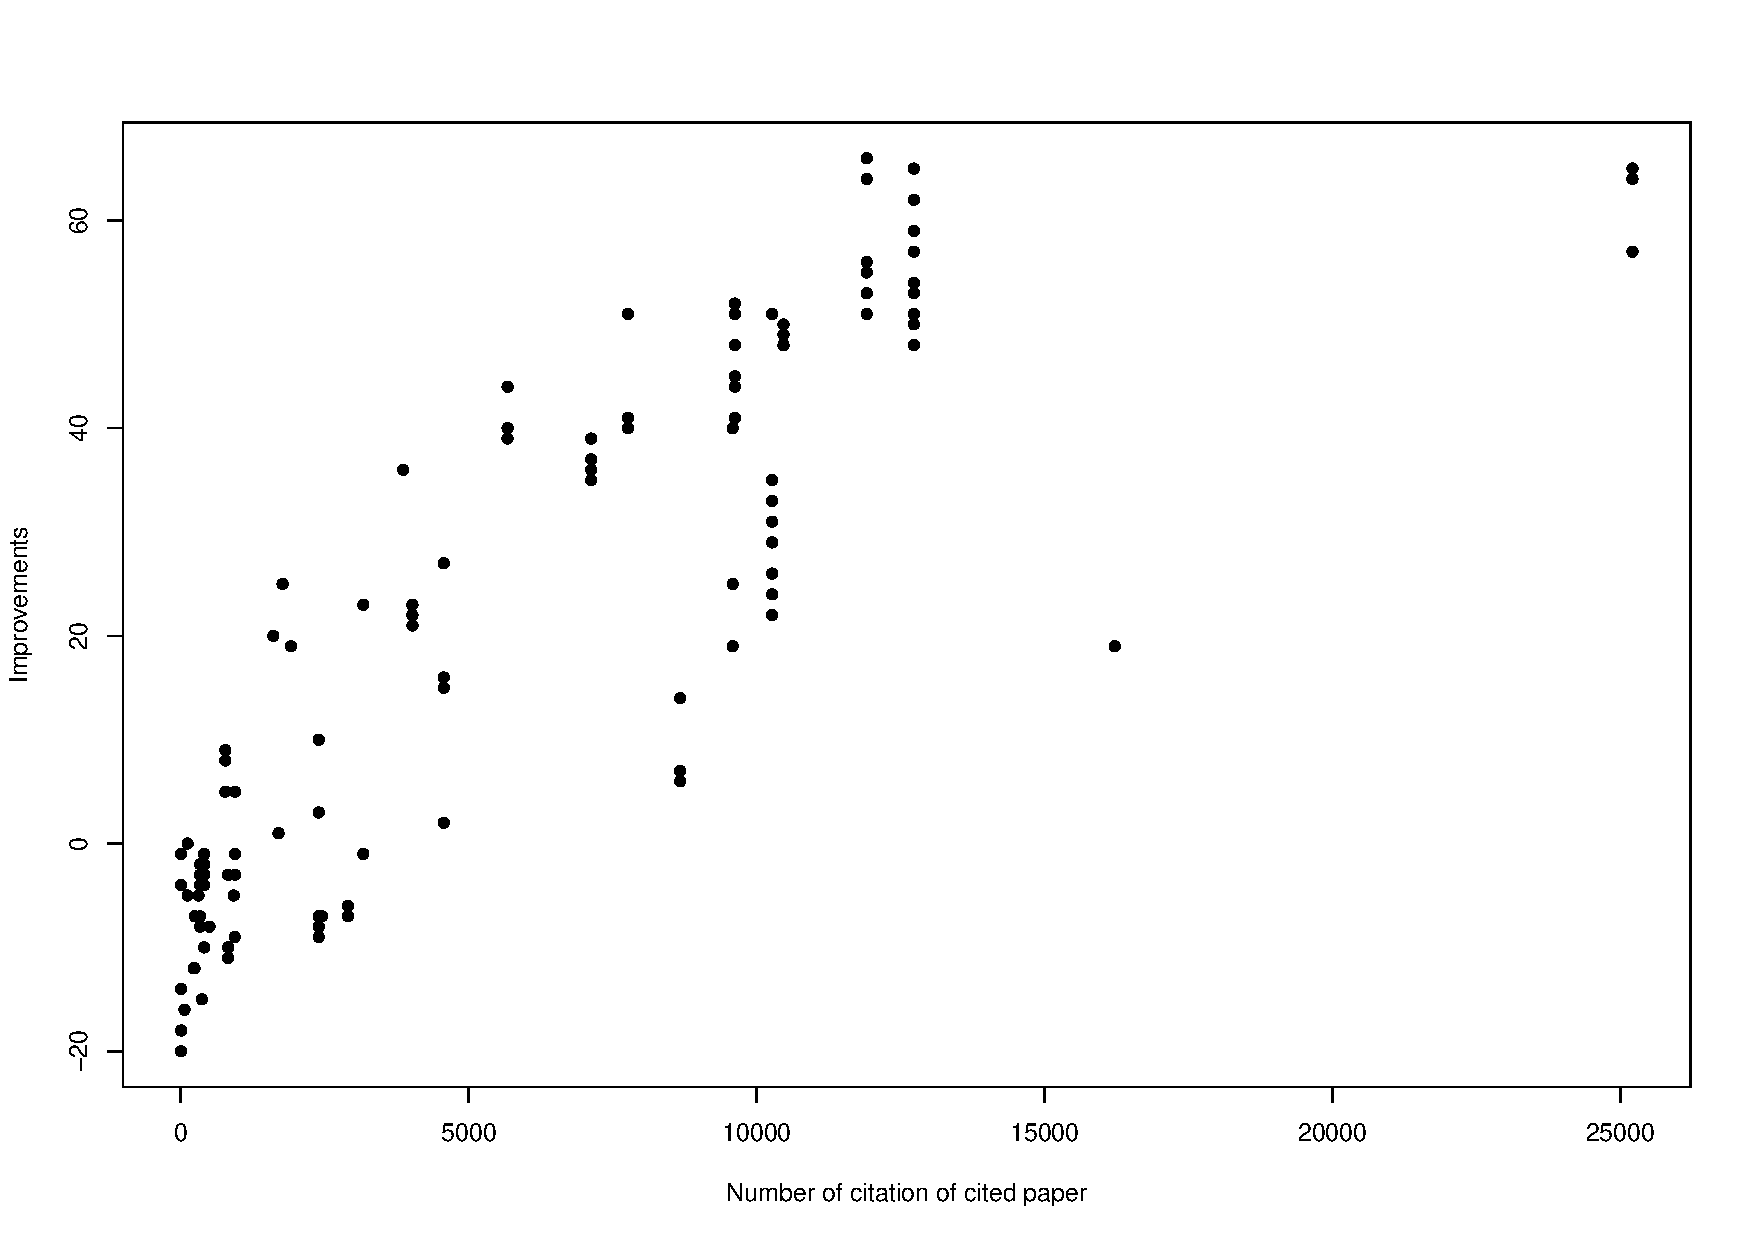
\includegraphics[width= \textwidth]{rq1_2.pdf}
\caption{Relation between ranking Improvements and citition count \label{fig:rq1_2}}
\end{figure}

Reminding motivation of the research, We tried to improve the ranking of highly cited paper. Figure~\ref{fig:rq1_2} shows that as the paper cited more, the improvement in ranking was greater.  The observation results about number of positive cases and negative cases and their effect size from Figure~\ref{fig:rq1}  can be re-observed in  \ref{fig:rq1_2}.


\subsection{Performance ob Small Data Set}

In the experiments, We used small size of training data. Using small training data, the ranking results of \npm shows worse than \npm's original paper\cite{Huang:2015:NPM:2886521.2886655}. In the experiments, in spite of the use of small input data, the technique of \name model improved the results. \name can compensate for the poor results  of \npm from lack of training data.


\section{Discussion}
\todo{BH}

\section{Conclusion}
\label{sec:Conclusion}
\todo{BH}


\bibliographystyle{splncs03}
\bibliography{ref}


\end{document}
